\section{Strumenti utilizzati}

\hspace{\parindent}Per la realizzazione della tesi sono stati usati i seguenti strumenti:
\paragraph{•} Arduino combinato con NFC Shield v2.0: formano il dispositivo per la lettura/scrittura degli abbonamenti
\paragraph{•} NFC Tag: dispositivo sul quale sono memorizzati gli abbonamenti
\paragraph{•} Java: linguaggio di programmazione con il quale è stata progettata l'interfaccia grafica per l'applicazione
\paragraph{•} NoSQL Database: database dove vengono salvati i dati degli utenti.

\subsection{Arduino Uno}
\hspace{\parindent} Arduino è una piattaforma hardware composta da una serie di schede elettroniche dotate di un microcontrollore. È stata ideata e sviluppata nel 2003 da alcuni membri dell'Interaction Design Institute di Ivrea come strumento per la prototipazione rapida e l'utilizzo in vari ambiti, per esempio la robotica e la domotica.
\begin{center}
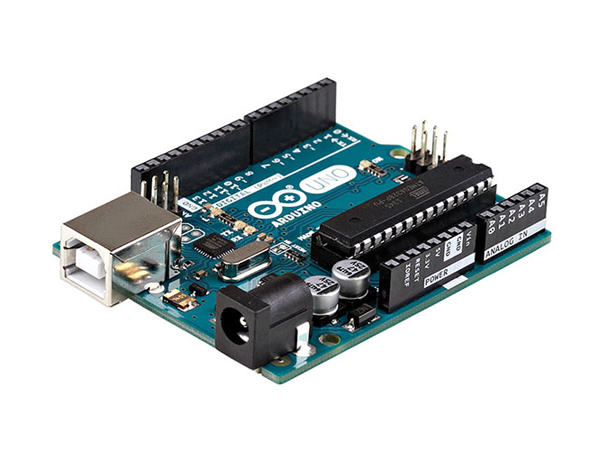
\includegraphics[scale=0.5]{arduino}
\end{center}
\subsection{NFC Shield v2.0}

\hspace{\parindent}Le shield sono schede che possono vengono inserite sopra l'Arduino, permettono l'estensione delle capacità della scheda stessa.La shield usata un questo progetto è quella NFC composta da un'antenna che collegandosi ad Arduino abilita la capacità di leggere/scrivere sui chip NFC
\begin{center}
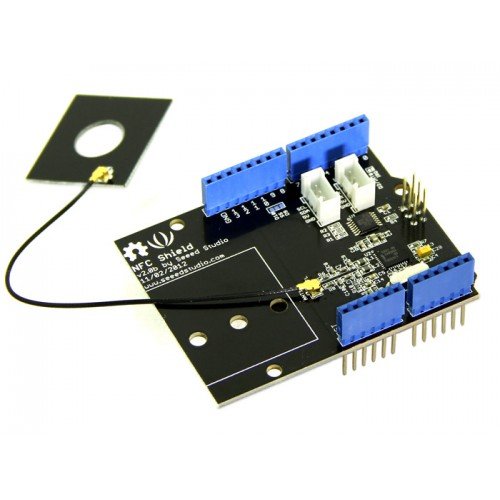
\includegraphics[scale=0.5]{shield}
\end{center}
\subsection{NFC Tag}
\hspace{\parindent}La tecnologia NFC  è una combinazione d'identificazione senza contatto (\textbf{RFID}) e altre tecnologie di connettività.NFC permette una comunicazione bidirezionale: quando due apparecchi NFC (initiator e target) vengono accostati entro un raggio di 4 cm, viene creata una rete peer-to-peer tra i due ed entrambi possono inviare e ricevere informazioni.
\\La tecnologia NFC opera alla frequenza di 13,56 MHz e può raggiungere una velocità di trasmissione massima di 424 kbit/s.
\\Il formato dei chip NFC usato nel progetto è \textbf{NDEF} 
\subsubsection{Tipologie di tag}
\hspace{\parindent}Prima di iniziare questa sezione è bene sapere che esistono solo cinque tipi di tag standardizzati e appunto per questo il loro funzionamento è garantito con gli accessori che possediamo in questo momento. I nuovi tipi di tag richiederanno una standaridzzazione e potrebbero anche richiedere un aggiornamento dell'architettura NFC che possediamo attualmente.

\paragraph{•}\textbf{Tipo 1}: il primo tipo è quello più semplice a causa di questo viene anche considerato come il più lento, ed essendo così semplice anche a livello di prezzo risulta essere molto economico. Il problema riguarda il fatto che certe funzionalità per delle applicazioni specifiche potrebbero mancare. Solitamente questi tag vengono usati per:
\subparagraph{-} Applicazioni in sola lettura
\subparagraph{-}  Accoppiamento di dispositivi bluetooth
\subparagraph{-} Lettura di un tag specifico quando c’`e ne sono tanti

\paragraph{•}\textbf{Tipo 2}:
Prima di iniziare questa sezione è bene sapere che esistono solo cinque tipi di tag standardizzati e appunto per questo il loro funzionamento è garantito con gli accessori che possediamo in questo momento. I nuovi tipi di tag richiederanno una standaridzzazione e potrebbero anche richiedere un aggiornamento dell'architettura NFC che possediamo attualmente.

\paragraph{•}\textbf{Tipo 3}: il terzo tipo si basa su standard differenti rispetto agli altri. Vengono anche conosciuti come i tag della Sony FeliCa, sono un'innovazione giapponese e molto usata in Asia. Offre molte funzionalità però il prezzo è molto alto, vengono appunto usati molto in Giappone e per questi tipi di applicazioni:
\subparagraph{-} Biglietti
\subparagraph{-} Moneta elettronica
\subparagraph{-} Dispositivi per l'assistenza sanitaria

\paragraph{•}\textbf{Tipo 4}: il quarto tipo di tag offre la maggior memoria e flessibilità tra tutti. Il prezzo è variabile però può aggirarsi dal medio all'alto, in funzione alla quantità di memoria che vuoi. La funzione più importante di questo tag è la \textit{sicurezza}, infatti è equipaggiato con funzionalità che permettono la "true authentication". Inoltre questo tag è l'unico che supporta lo standard ISO 7816 relativo alla sicurezza, inoltre permette l'auto-modifica del contenuto NDEF. Solitamente questo tag viene usato per applicazioni di biglietteria.

\paragraph{•}\textbf{Tipo 5}: il quinto tipo offre supporto per la specifica ISO 15693, viene supportata la Modalità di Comunicazione Attiva, che permette di ottenere performance in ambito di trasferimento dei dati simili alle tecnologie RF. La distanza di lettura è uguale a quella degli altri tag NFC, solitamente questi tag vengono usati per:
\subparagraph{-} Impacchettamento di prodotti
\subparagraph{-} Biglietti
\subparagraph{-} Dispositivi per l'assistenza sanitaria

\subsubsection{Standard ISO}
\hspace{\parindent}Ci sono diversi standard ISO usati per la tecnologia NFC tra cui: ISO 15693, 18092 e 21481 poi ECMA 340, 352 e 356 ed ETSI TS 102 190. NFC è inoltre compatibile con la diffusa architettura delle smart card contactless, basate su ISO 14443 MIFARE e Sony FeliCa (tipo 4).

\paragraph{•} ISO 15693: Lo standard ISO 15693 utilizza la frequenza 13.56 MHz, viene offerta una distanza di lettura che può variare tra 1 metro ed 1.5 metri, poiché le carte devono operare a distanza, è richiesta la presenza di campi magnetici inferiori rispetto a quelli usati per altre carte. Inoltre a differenza di altri standard c'è una funzione di anticollisione implementata, questo serve per consentire una lettura simultanea di più card senza incorrere in errori o fail di ricezione.
\paragraph{•} ISO 18092, definisce lo standard di una smartcard contactless, viene prevalentemente usato nei sistemi RFID (pre-NFC). Questa tecnologia  viene usata con i tag di tipo 4 quindi in Giappone. Questa specifica è formata dalle ISO 15693 (vista prima) e dalla ISO 9798 che regolamenta il protocollo di comunicazione a mutuo riconoscimento, questo implica che il tag può essere letto solo da un lettore già programmato.

\subsection{NoSQL Database}
\hspace{\parindent} I database NoSQL (non relazionali), sono realizzati per modelli di dati specifici, hanno degli schemi flessibili, un'ottima facilità di sviluppo, una scalabilità orizzontale e delle prestazioni ottime. Si può pensare all'attuale diffusione dei sistemi cloud, quindi una diffusione dove ci sono moltissimi nodi e usare un RDMBS (database relazionale) in questi casi diventerebbe molto difficile. I principali metodi d'implementazione dei database NoSQL sono:
\paragraph{•}Chiave-valore: I dati sono immagazzinati in un elemento che contiene una chiave oltre che i dati veri e propri, dal punto di vista implementativo questo è il metodo più semplice, però è anche quello meno efficiente nel caso nel quale le operazioni riguardano solo una parte dell'elemento e non l'elemento nel totale 
\paragraph{•}Column family: i dati vengono organizzati in righe e colonne, non si ha il bisogno di definire il numero di colonne e una riga può avere molte colonne
\paragraph{•}Document store: è un'evoluzione del metodo chiave-valore, i dati vengono salvati in un documento che può contenere un numero "infinito" di campi di "infinita" lunghezza, in questo modo riusciamo ad evitare sprechi di campi inutilizzati che andrebbero ad occupare spazio in memoria.

\subsection{WindowBuilder}
\hspace{\parindent}Per la realizzazione dell'interfaccia grafica in Java è stato usato il plug-in WindowBuilder di Eclipse. Questo plug-in è composto a partire dalle liberire SWT Designer e Swing Designer e rende comoda e veloce la creazione di interfacce grafiche (GUI) per le applicazioni Java. Usando il WYSIWYG visual designer e gli strumenti di layout è possibile creare finestre complesse, e per ogni elemento messo verrà generato il codice contente la posizione dell'elemento e la sua dichiarazione.
\\Inoltre, il codice generato da questa libreria non richiede l'uso di altre librerie personalizzate per compilarlo ed eseguirlo, inoltre è possibile dall'interfaccia grafica creare eventi che poi andranno compilati mediante codice scritto in dei blocchi di \textit{ActionListener}, è possibile generare diversi tipi di eventi, dal click del mouse, alla pressione di un tasto sulla tastiera, o persino al movimento nella finestra del mouse.

\subsection{Cassandra}
\hspace{\parindent}Apache Cassandra è un DBMS distribuito e open source. Si tratta di un progetto Top-Level, sviluppato da Apache Software Foundation per gestire grandi quantità di dati dislocati in diversi server, fornendo un servizio orientato alla disponibilità.
\\È una soluzione NoSQL che inizialmente fu sviluppata da Facebook, un modello di dati simile a BigTable in esecuzione su un'infrastruttura tipi Amazon-Dynamo. Cassandra fornisce una struttura di memorizzazione chiave-valore, con Eventual Consistency.
\begin{center}
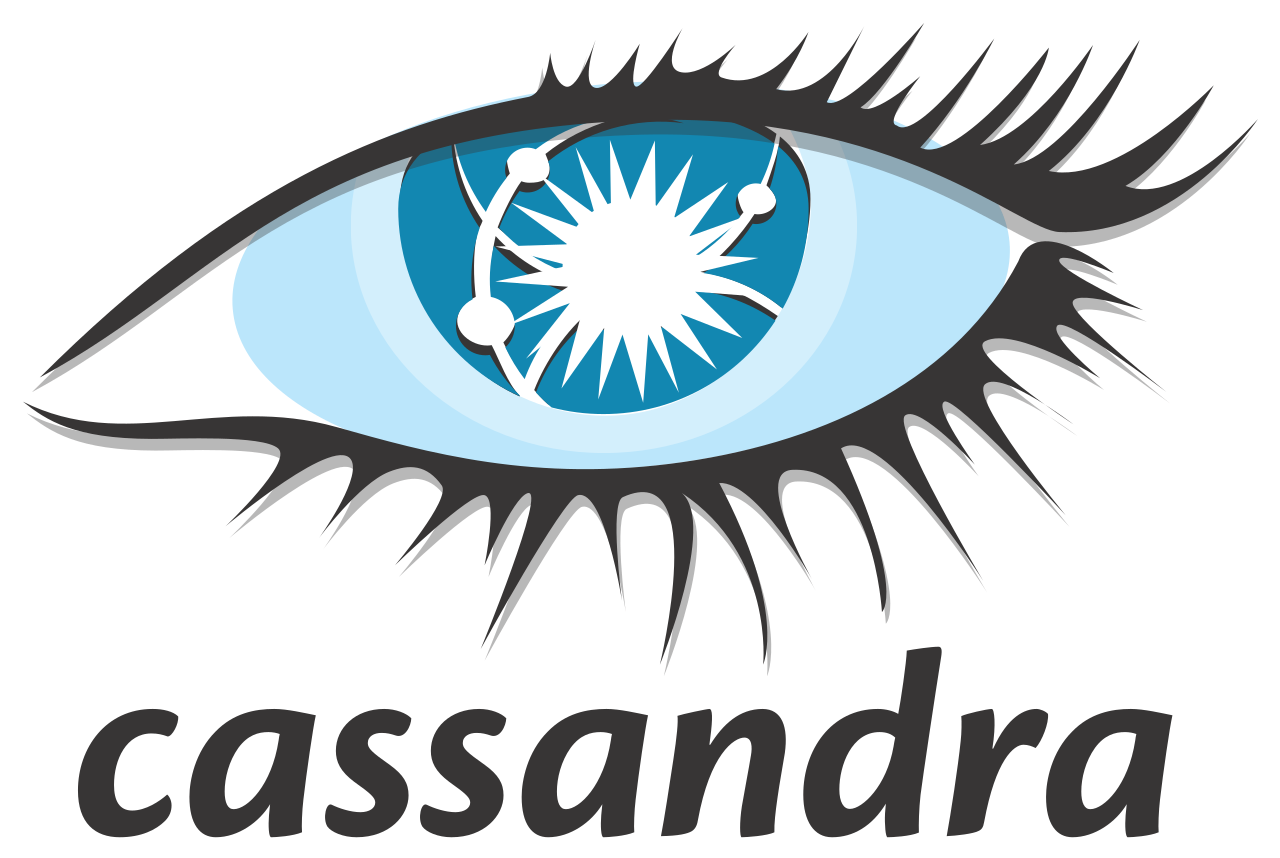
\includegraphics[scale=0.15]{cassandra}
\end{center}
Alle chiavi corrispondono dei valori, raggruppati in famiglie di colonne: una famiglia di colonne è definita quando il database viene creato. Tuttavia le colonne possono essere aggiunte a una famiglia in qualsiasi momento.
\\Le colonne sono aggiunte solo specificando le chiavi, così differenti chiavi possono avere differenti numeri di colonne in una data famiglia. I valori di una famiglia di colonne sono memorizzati insieme, questo perché Cassandra adotta un approccio ibrido tra DBMS orientato alle colonne e la memorizzazione orientata alle righe.
\\Come caratteristiche principali abbiamo:
\paragraph{•} Fault-tolerance: i dati vengono replicati in maniera automatica su più nodi, la replica è supportata tramite vari data center e la sostituzione dei nodi può avvenire senza downtime\footnote{la replicazione verrà trattata nel capitolo 3.4.2}.
\paragraph{•} Tunable consistency: il livello di coerenza può essere modificato (da writes never fail a block for all replicas to be readable).
\subsubsection{CQLSH}
\hspace{\parindent}cqlsh\footnote{http://cassandra.apache.org/doc/latest/tools/cqlsh.html} è una shell a linea di comando per interagire con Cassandra attraverso il CQL (Cassandra Query Language), è inclusa con ogni versione di Cassandra, questa shell utilizza dei protocolli nativi di Python e permette la connessione al nodo specificato nella linea di comando \footnote{un esempio di connessione sarà trattato nel capitolo 3.4.4}.
\\Generalmente parlando, il funzionamento di una data versione di cqlsh  è garantito solo con la versione di cassandra che lo ha rilasciato, ci possono essere casi particolari nei quali vengono rilasciati update per far lavorare un cqlsh datato con una nuova versione di Cassandra, però questo non è supportato ufficialmente.